% !TEX program = xelatex
% ICLC 2027 live-performance proposal — papers-stack edition.
% Follows the ICLC template structure (general info → description → media →
% program note → bio → technical questionnaire) so reviewers find every
% required section where they expect it.
\documentclass[10pt,letterpaper]{article}
\usepackage[top=0.85in, bottom=0.85in, left=1in, right=1in, footskip=14pt]{geometry}

% === FONTS (papers-stack pattern: OTF filenames, never font names) ===
\usepackage{fontspec}
\setmainfont{Latin Modern Roman}[
 Extension=.otf,
 UprightFont=lmroman10-regular,
 BoldFont=lmroman10-bold,
 ItalicFont=lmroman10-italic,
 BoldItalicFont=lmroman10-bolditalic,
]
\setsansfont{Latin Modern Sans}[
 Extension=.otf,
 UprightFont=lmsans10-regular,
 BoldFont=lmsans10-bold,
 ItalicFont=lmsans10-oblique,
 BoldItalicFont=lmsans10-boldoblique,
]
% YWFT Processing: display title ONLY; punctuation set in \normalfont escapes.
\newfontfamily\acbold{ywft-processing-bold}[
 Path=../../system/public/type/webfonts/,
 Extension=.ttf
]

\usepackage{xcolor}
\definecolor{ink}{HTML}{1B1B2E}
\definecolor{acred}{HTML}{C2185B}
\definecolor{fog}{HTML}{6E6E82}
\usepackage{graphicx}
\graphicspath{{figures/}}
\usepackage[hidelinks]{hyperref}
\usepackage{xurl}
\usepackage{parskip}
\usepackage{titlesec}
\usepackage{tikz}
\usepackage{caption}
\captionsetup{font={small,it},labelfont={small,bf},skip=6pt}
\titleformat{\section}{\large\bfseries\sffamily\color{ink}}{\thesection.}{0.5em}{}
\titleformat{\subsection}{\normalsize\bfseries\sffamily\color{ink}}{\thesubsection}{0.5em}{}
\titlespacing{\section}{0pt}{14pt}{6pt}
\titlespacing{\subsection}{0pt}{10pt}{3pt}
\pagestyle{plain}
\color{ink}

\begin{document}

% ===== title block =====
\begin{center}
{\acbold\fontsize{30pt}{34pt}\selectfont NOTE{\normalfont\bfseries(}S{\normalfont\bfseries)}PAT{\normalfont\bfseries(}IAL{\normalfont\bfseries)} NATIVE\par}
\vspace{6pt}
{\large twelve sound bodies on six surplus laptops\par}
\vspace{4pt}
{\small\color{fog}ICLC 2027 --- proposal for live performances \ · \ concert format \ · \ one performer \ · \ $\sim$15 minutes\par}
\end{center}

\vspace{4pt}
\begin{figure}[h]
\centering
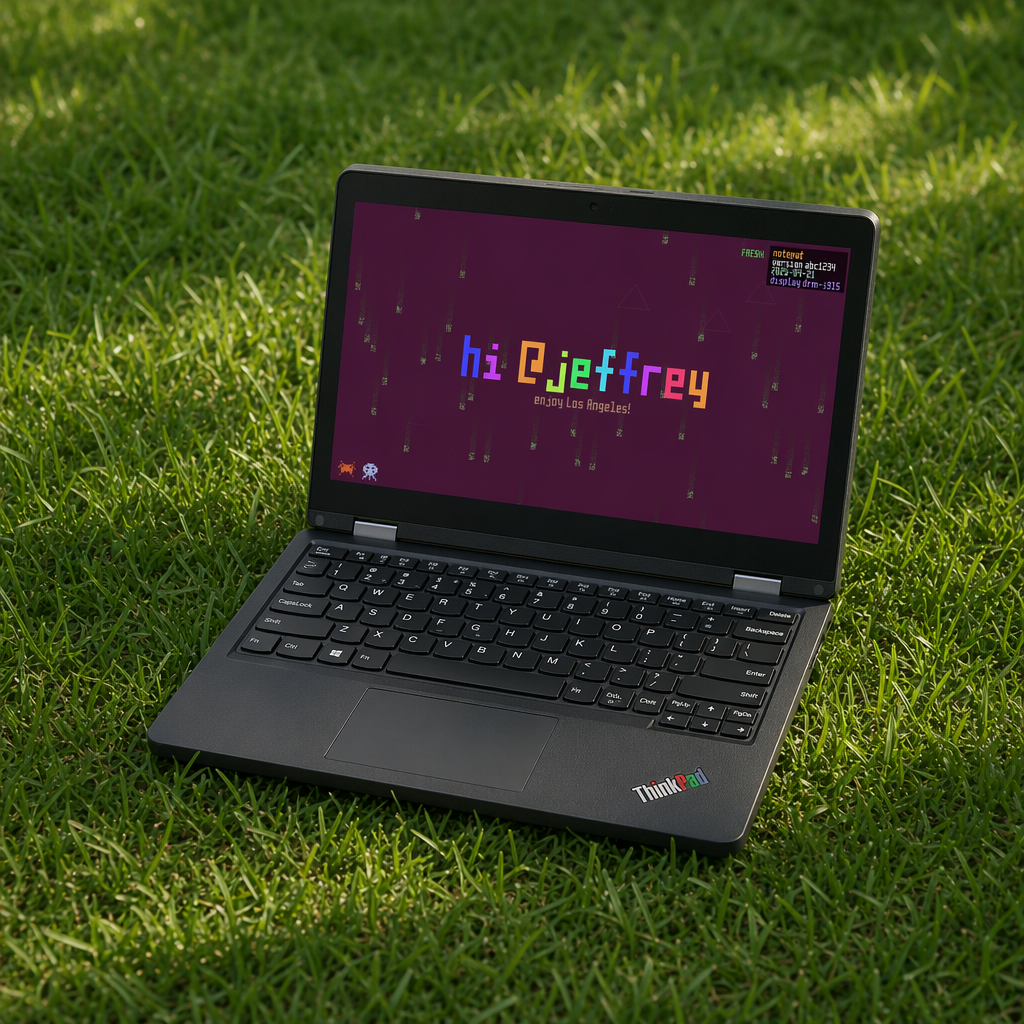
\includegraphics[width=0.78\linewidth]{ac-native-laptop.png}
\caption{The instrument, singular: a surplus ThinkPad booted from USB into
AC Native, the bare-metal build of Aesthetic Computer, running the notepat
instrument. Six machines of this kind, placed among the audience, form the
loudspeaker orchestra.}
\end{figure}

\section{General Information}

\textbf{Performance title:} Note(s)pat(ial) Native --- twelve sound bodies on six surplus laptops\\
\textbf{Main contact:} Jeffrey Alan Scudder, Aesthetic Computer, Los Angeles --- \texttt{mail@aesthetic.computer}\\
\textbf{Additional performers:} none (solo)\\
\textbf{Performance type:} Concert --- seated or freely moving audience, interleaved with the loudspeaker-laptops

\section{Performance Description}

Note(s)pat(ial) Native is a fifteen-minute spatial performance in which the
loudspeaker orchestra is a fleet of surplus grade-school laptops, each booted
from USB into a bare-metal creative operating system and each responsible for
one channel of the room. The audience sits inside the array. Twelve moving
sound bodies --- sustained tones, percussion, and bass that orbit, approach,
and recede --- are grown live from a fixed 1:41 composition, and a single
performer at a control surface turns the whole field, changes its speed, and
hands individual voices from machine to machine while the room listens from
the middle.

The material is fully computed and fully known: the source composition is
rendered by a deterministic engine whose 1,932 events constitute the score
(Figure~\ref{fig:score}). Each laptop receives only the events for its
assigned bodies and renders them locally; there is no mixing desk and no
house PA in the loop. The machines agree on a shared downbeat by estimating
clock offset against a common reference (Cristian's algorithm,
millisecond-scale residual), and all in-performance control travels over a
local network the piece carries with it --- the work has no dependency on
venue infrastructure beyond power. What is live is the conducting of the
computation itself: rotation of the spatial field, elastic time, and the
reassignment of voices between machines are performed, not played back, so
no two rooms hear the same realization.

\begin{figure}[t]
\centering
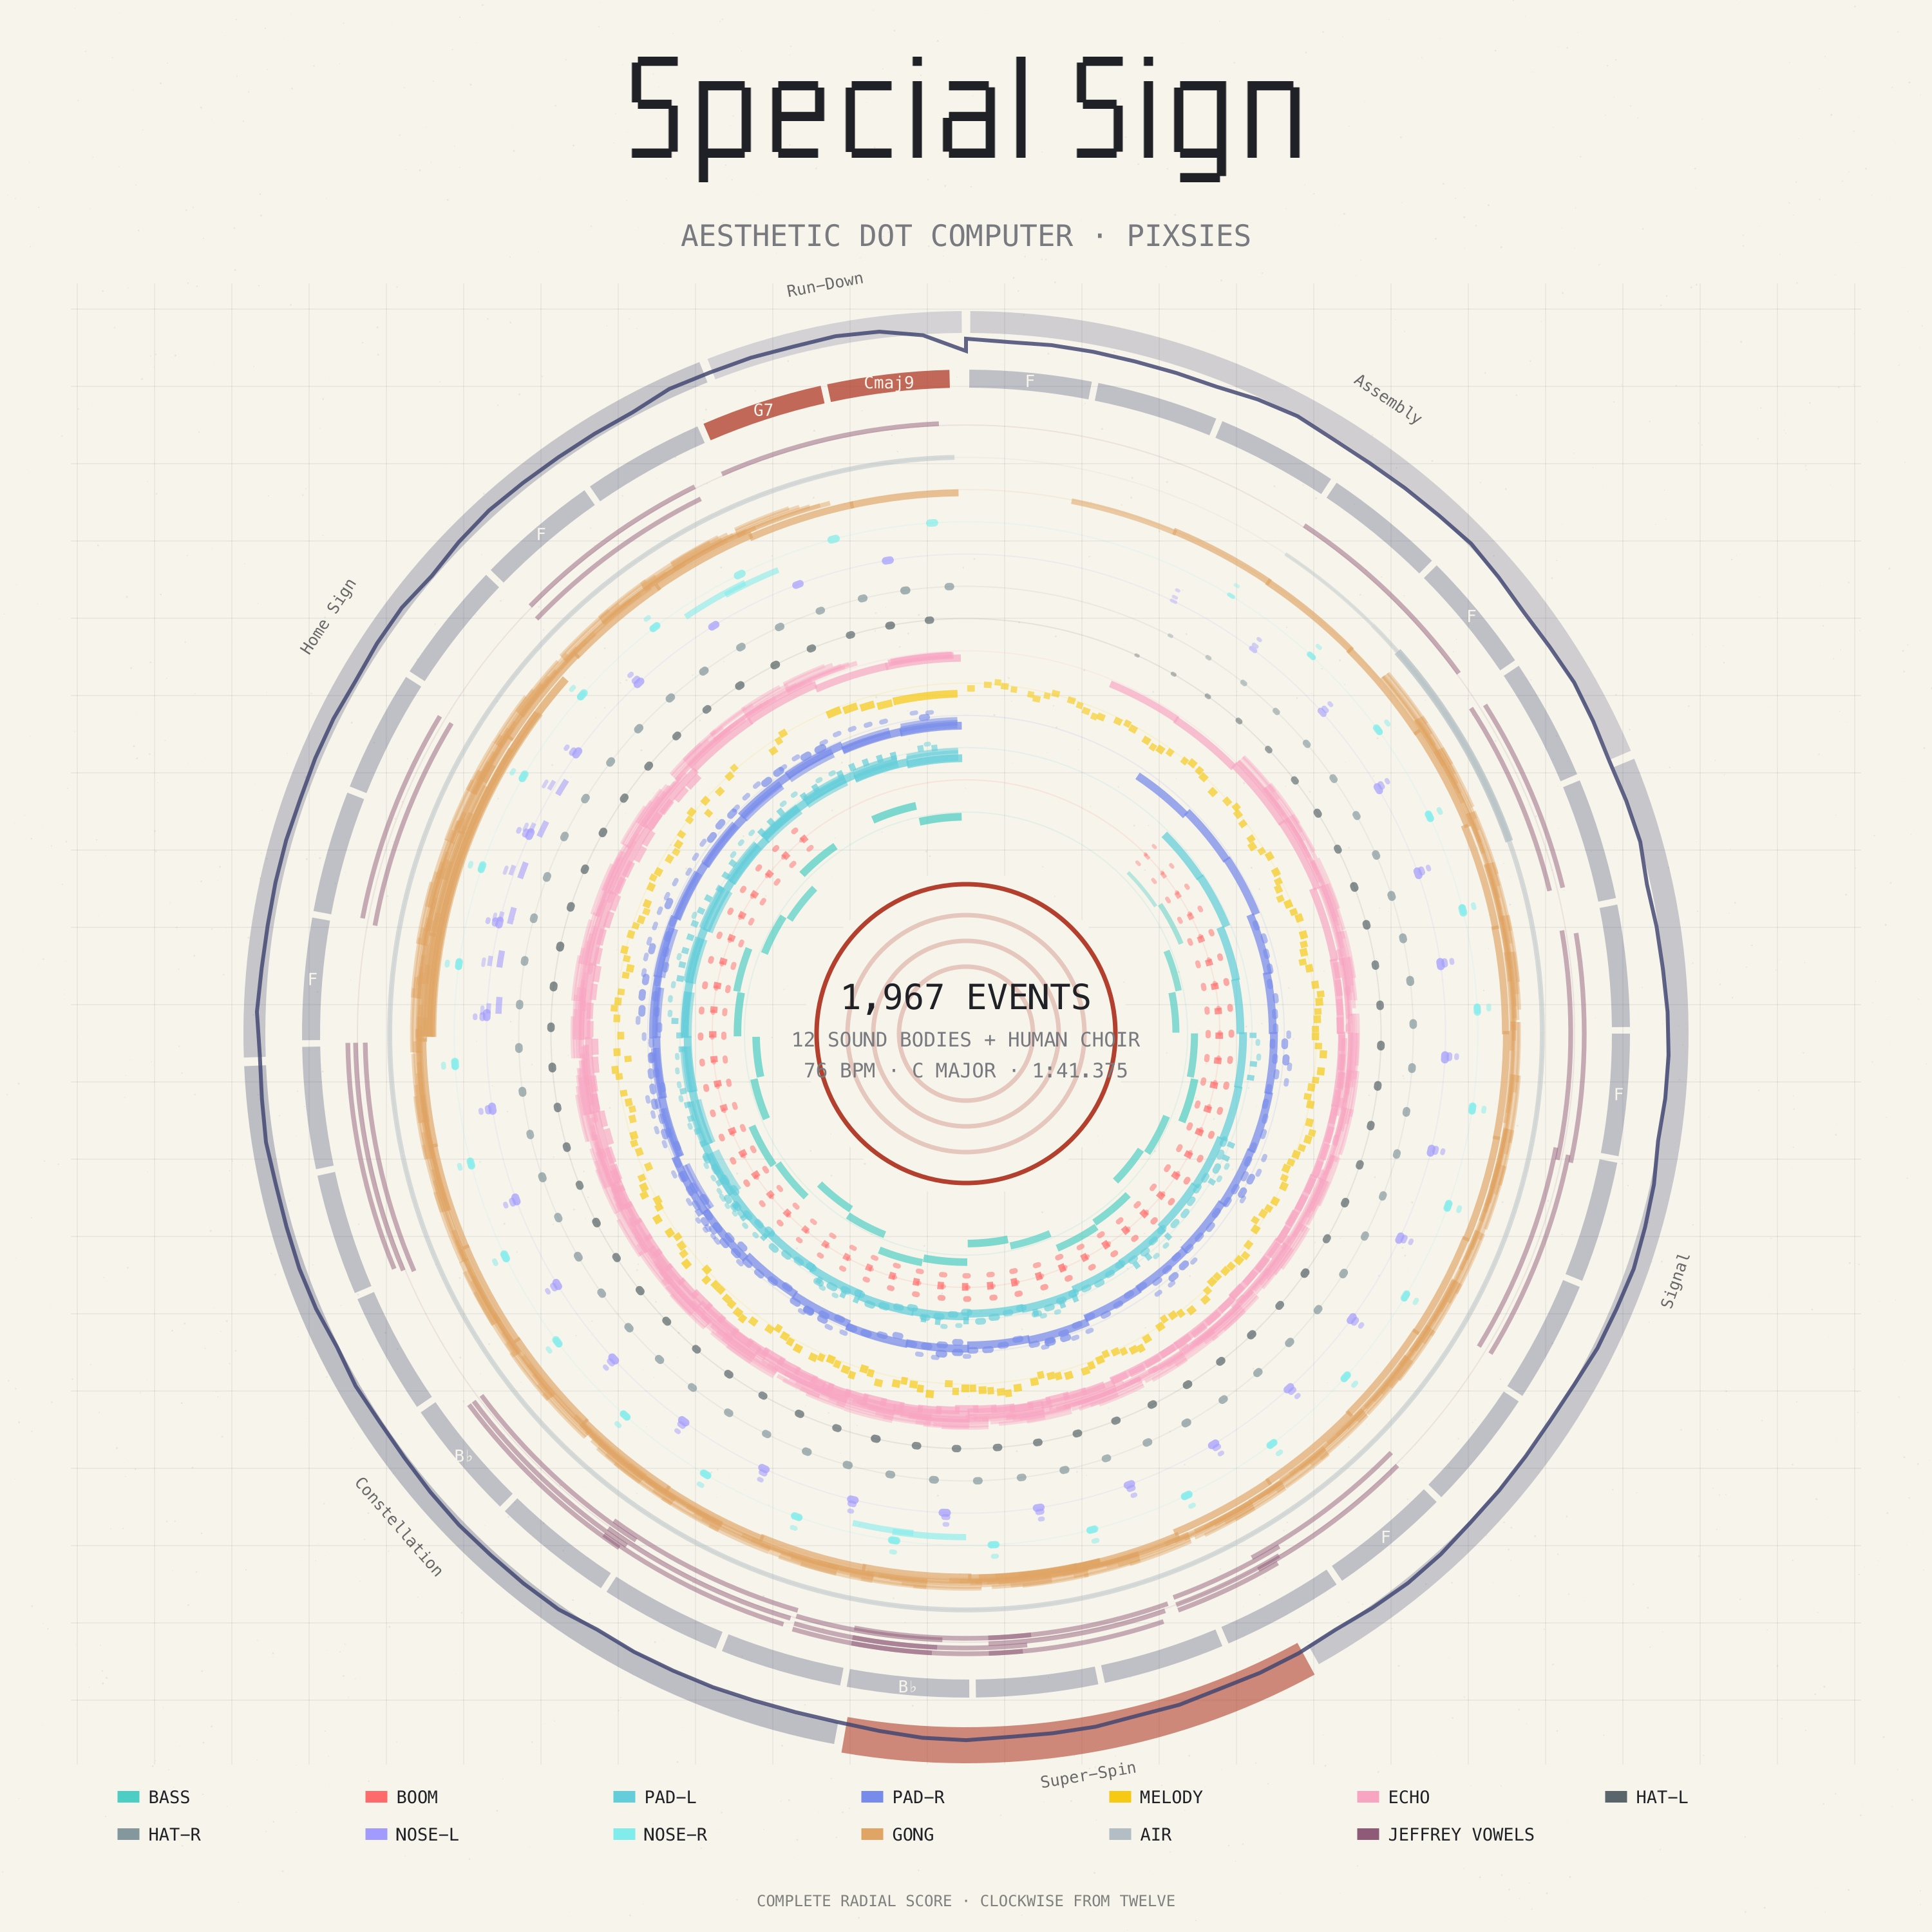
\includegraphics[width=0.62\linewidth]{special-sign-radial-score.jpg}
\caption{The score as a complete radial figure: thirteen colored orbits
carrying the engine's 1,932 events plus 35 choir events, movement and chord
rings wrapping clockwise around the dynamic arc. The performance grows this
fixed 1:41 field into $\sim$15 minutes of conducted space.}
\label{fig:score}
\end{figure}

The piece is built as three reciprocal loops, which is why it belongs to
\emph{Dialogues}. The first is performer-to-field: the conductor is steering
a computation in flight, and the field answers with the acoustics of the
actual room, so every gesture is a question asked of a space. The second is
machine-to-machine: the central performable gesture is the handoff, in which
a voice leaves one named, physical, second-hand computer and arrives in
another across the room (Figure~\ref{fig:room}) --- a conversation between
specific machines the audience can point at, not between abstract channels.
The third is field-to-audience: because the diffusion bodies are discrete
objects scattered among listeners rather than a ring of monitors at the
perimeter, each listener's position is their own mix, and moving one's head
is a form of participation the piece anticipates rather than tolerates.

There is also a quieter dialogue running underneath: with the institutional
discard pile. The six machines are surplus school laptops of the kind
retired by districts in bulk. The operating system boots from a USB stick
and changes nothing on their disks; the piece borrows the machines rather
than consuming them, and after the performance they remain what they were.
Presenting obsolete public-education hardware as a precision spatial
instrument is the work's argument in physical form: personal computers are
not done yet, and an instrument can live inside a computer the way a clock
does --- as a built-in facility, not an application someone must go and get.

The system is part of Aesthetic Computer, an open-source creative computing
environment developed by the author since 2021, whose instruments (the
notepat keyboard instrument, Figure~\ref{fig:notepat}, and the KidLisp
live-coding language among them) are addressable as URLs and playable in the
room by anyone. Within the live coding tradition the work is positioned
honestly: the score is source code and the performance is its evaluation
steered live, closer to conducted computation than to projected-text
livecoding. Its ancestors include the loudspeaker-orchestra diffusion
practice of the acousmatic tradition and the laptop-orchestra lineage of
PLOrk and SLOrk; it differs from both in that the diffusion instrument is
the fleet itself --- commodity machines, one channel each, no performer
seated at any of them --- and in that the material is a fixed,
pop-song-length composition whose liveness is spatial and temporal rather
than notational.

\begin{figure}[t]
\centering
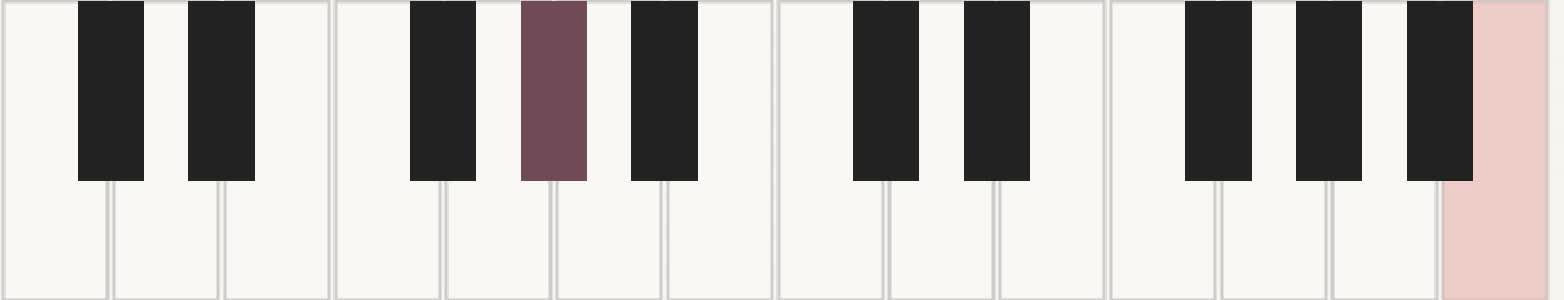
\includegraphics[width=\linewidth]{notepat-keyboard.jpg}
\caption{notepat, the Aesthetic Computer keyboard instrument, as it boots in
any browser at \texttt{aesthetic.computer/notepat} --- the same instrument
that runs natively on each performance machine.}
\label{fig:notepat}
\end{figure}

The performance premieres at CultureHub Los Angeles on September 24, 2026,
as half of an evening of new work for revived hardware; documentation of
that premiere will be available well before the review period concludes. The
piece is one performer, approximately fifteen minutes, and scales from four
to eight machines to fit the room, all hardware and networking carried by
the artist. In keeping with ICLC's disclosure policy: the performance
system, composition, and engine are the author's; large-language-model
assistance was used in preparing the text of this proposal.


\section{Video and/or Audio Material}

\begin{itemize}
  \item \url{https://assets.aesthetic.computer/pop/special-sign/special-sign-sine-system-reel.mp4}
        --- motion documentation of the source composition's sine-system engine (38 s, with audio).
  \item \url{https://aesthetic.computer} --- the live system; instruments run in the browser.
  \item \url{https://aesthetic.computer/notepat} --- the notepat instrument, playable now.
  \item \url{https://github.com/whistlegraph/aesthetic-computer} --- open source, full history.
  \item Documentation of the September 24, 2026 CultureHub Los Angeles premiere
        (video) will be published at \url{https://aesthetic.computer} ahead of the
        review period.
\end{itemize}

\section{Program Note}

Six surplus grade-school laptops sit among the audience, each booted from a
USB stick into a bare-metal creative operating system, each speaking one
channel of the room. Twelve sound bodies --- tones, percussion, bass --- are
grown live from a fixed 1:41 composition: they orbit, approach, and recede,
and a single performer turns the field, stretches its time, and hands voices
from machine to machine. There is no PA; the computers are the orchestra,
and every seat hears its own mix. The machines are borrowed, not consumed
--- the stick changes nothing on their disks, and after the piece they
remain retired school laptops. The work is part of Aesthetic Computer, an
open-source environment built on the conviction that an instrument belongs
inside a computer the way a clock does. First performed at CultureHub Los
Angeles, September 2026.

\section{Artist Biography}

Jeffrey Alan Scudder (b.\ 1989, USA) is an artist and toolmaker who has
developed Aesthetic Computer, an open-source creative computing environment,
in continuous public practice since 2021. His software performances and
drawing systems have been presented by the New Museum's Rhizome (commission,
2022), Feral File, and venues and classrooms internationally; earlier tools
include Plotato and the Whistlegraph drawing-performance practice, made with
the collective of the same name. He holds an MFA from Yale (2013) and a BFA
from Ringling College of Art and Design (2011), and has taught creative
computing at institutions including UCLA. His current work revives surplus
and obsolete hardware as musical instruments: laptops flashed into a
bare-metal creative OS whose instruments are addressable as URLs and
playable by anyone. He performs as a resident artist at CultureHub Los
Angeles in September 2026. He lives and works in Los Angeles.

\vspace{10pt}
\begin{figure}[h]
\centering
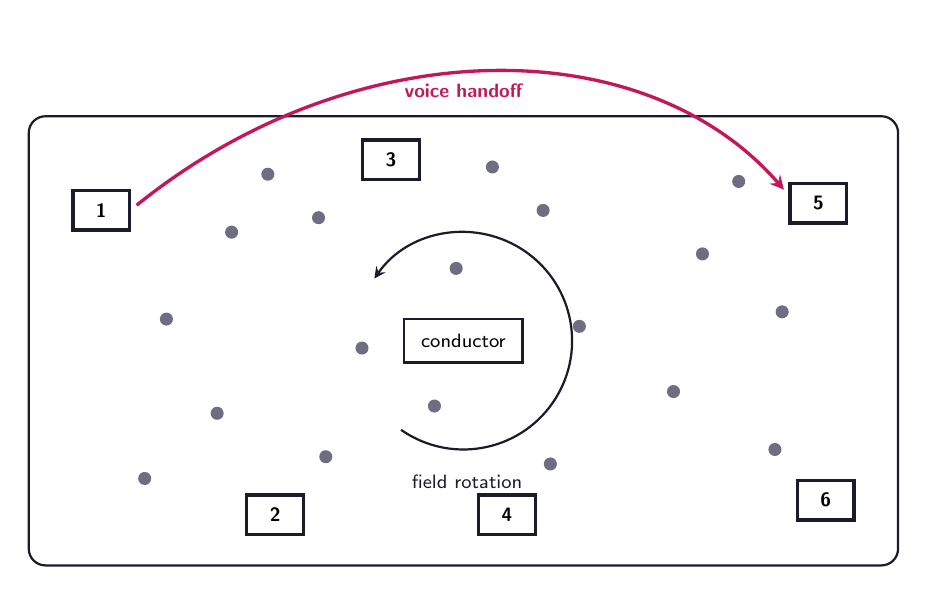
\begin{tikzpicture}[x=1cm,y=1cm,scale=0.92]
  % room
  \draw[ink, thick, rounded corners=6pt] (0,0) rectangle (12,6.2);
  % audience dots
  \foreach \p in {(1.6,1.2),(2.6,2.1),(1.9,3.4),(2.8,4.6),(4.1,1.5),(4.6,3.0),
                  (4.0,4.8),(5.6,2.2),(5.9,4.1),(7.2,1.4),(7.6,3.3),(7.1,4.9),
                  (8.9,2.4),(9.3,4.3),(10.3,1.6),(10.4,3.5),(9.8,5.3),(3.3,5.4),(6.4,5.5)}
    \fill[fog] \p circle (0.09);
  % six machines
  \foreach \pos/\n in {(1.0,4.9)/1,(3.4,0.7)/2,(5.0,5.6)/3,(6.6,0.7)/4,(10.9,5.0)/5,(11.0,0.9)/6}{
    \node[draw=ink, very thick, fill=white, minimum width=0.72cm, minimum height=0.5cm, inner sep=1pt] at \pos {\scriptsize\sffamily\bfseries \n};
  }
  % performer table
  \node[draw=ink, thick, fill=white, minimum width=1.5cm, minimum height=0.55cm] at (6.0,3.1) {\scriptsize\sffamily conductor};
  % handoff arc: machine 1 -> machine 5
  \draw[acred, very thick, -{stealth}, shorten >=3pt, shorten <=3pt]
    (1.4,4.9) .. controls (4.5,7.4) and (8.5,7.4) .. (10.5,5.1);
  \node[acred, font=\scriptsize\sffamily\bfseries] at (6.0,6.55) {voice handoff};
  % rotation arrow
  \draw[ink, thick, -{stealth}] (6.0,3.1) ++(-125:1.5) arc (-125:145:1.5);
  \node[font=\scriptsize\sffamily, text=ink] at (6.05,1.15) {field rotation};
\end{tikzpicture}
\caption{The room as instrument: six loudspeaker-laptops (1--6) distributed
through the audience (dots), a single conductor mid-room, the spatial field
rotating around the listeners, and a voice handed live from machine 1 to
machine 5 across the space. Layout scales from four to eight machines.}
\label{fig:room}
\end{figure}

\newpage

\begin{center}
{\acbold\fontsize{22pt}{26pt}\selectfont TECHNICAL REQUIREMENTS\par}
\vspace{2pt}
{\small\color{fog}ICLC 2027 --- live performances questionnaire\par}
\end{center}

\section{General Information}

\subsection{What setting is the performance intended for?}
Concert setting, indoors. Ideal: flexible/cabaret seating with the six
loudspeaker-laptops placed \emph{among} the audience --- listeners inside
the array, free to turn or move. Raked rows work if the machines can be
distributed around and within the seating. Dim, calm lighting with one warm
special on the performer table is ideal; lighting is nice-to-have, not a
showstopper. The only absolute requirement is distributed power.

\subsection{How many performers will be in the performance?}
One.

\subsection{Are you open to being paired with another performer?}
No --- the piece is a complete spatial-audio work and the room of machines
is its visual; projected visuals would compete with the physical field.

\subsection{Will your performance require technical support during the set?}
No. A single preset lighting state is enough; no cues during the set.

\section{Materials Needed}

\subsection{What are your projection needs?}
None. No projection is used.

\subsection{How many input channels on the mixing console do you need?}
Zero for the performance --- there is no house PA in the signal path. If the
venue wants an archival or stream feed, I can provide a stereo pair
(2$\times$ XLR or \textonequarter{}'') from a monitoring mix; optional.

\subsection{Do you require a microphone?}
Not for the piece. One announce/talkback microphone for a spoken
introduction is welcome if the house has one; optional.

\subsection{Do you require a monitor, either over headphones or otherwise?}
No.

\subsection{Are you bringing your own audio interface?}
Not applicable --- the six laptops render and emit all audio themselves; no
interface or house audio path is required.

\subsection{How much table/floor space will you need? How many chairs?}
One performer table ($\sim$120 $\times$ 60 cm) and one chair. Six small
tables, plinths, or stools ($\sim$40 $\times$ 40 cm each) distributed
through the audience area for the laptops. Footprint scales to the room.

\subsection{Do you need an internet connection during the performance?}
No. The piece carries its own closed local network (artist-provided
router/switch); it has no dependency on venue Wi-Fi or Ethernet.

\subsection{Anything else you need?}
Six to eight distributed power outlets (or permission to run artist-provided
power strips and extension cables through the seating area). Everything else
--- laptops, USB boot media and spares, network hardware, cabling --- is
carried by the artist. Setup 90 minutes, strike 30 minutes.

\end{document}
